%!TEX root = ../thesis.tex

\chapter{BEM with inexact GMRES for Red Blood Cell problems}\label{chapter:rbc}
\thispagestyle{myheadings}

\graphicspath{{RBC/}}

To show ``real-world'' performance, we choose an application closer to contemporary Stokes {\bem} research than flow past a sphere. The behavior of both flow past red blood cells (RBCs), in our case ethrocytes, and the effect of this flow on the cells themselves has prompted research based on a variety of methods, from traditional fluid solvers to boundary integral formulations like the one presented in this thesis. These studies are of particular use to the medical field --- by better understanding the microcirculation of blood, topics such as anti-coagulation therapy and stroke research would greatly benefit \cite{RahimianETal2010}. To summarize state-of-the-art in the boundary integral representation of RBCs, we briefly discuss 3 papers.

The first was an early attempt at a large-scale simulation \cite{zinchenko2003}, using $\O{1000}$ panels per elliptical cell (Vessicle) and utilizing a periodic domain of $\O{100s}$ of cells in order to approximate blood cells in plasma using an emulsion model. Extending this idea, the winner of the prestigious Gordon Bell prize in 2011 \cite{RahimianETal2010} used large numbers of low-definition elliptical vessicles ($\O{100}$ panels per cell) with a coupled Stokes and elasticity formulation to simulate blood drops -- the largest simulation was performed with 200 million cells, and 90 billion unknowns (velocity and forces). This corresponds to roughly 40 drops of blood. Finally, the simulation closest in capability to the work in this thesis involves 40 ethrocyte cells comprising of 7500 panels each \cite{Liu2009}. This experiment was non time-dependant, and did not involve any cell deformation, making it directly comparable to our work.

These experiments are characterized by their size --- the computational capacity required, the number of cells used and the amount of time taken for simulations. The application of a relaxation scheme would give the option of either reducing both the computational and time requirements, or performing experiments with more cells or the same amount, but better discretized cells. Both options would provide a significant gain in capability for any suitable code.

While research often includes deformation of the cells by using a linear elasticity {\bem} and unsteady flow to show the time-dependant evolution of cells in blood flow, we choose to demonstrate only the Stokes-flow part. The equations for linear elasticity can be treated in the same way as those for the Stokes equation --- we integrate over tensors, the result is a vector quantity, and we can use an {\fmm} to improve the scaling of $N$-body products by a decomposition into multiple harmonic {\fmm}s. Thus, speedups from relaxation for the purely Stokes problem can be viewed as analogous to speedups that would be required for both linear elasticity and the combined problem. Unsteady flow would involve repeated {\bem} solves of comparable or equal difficulty, so we can view any speedup for a single solve (single time-step) as applicable for every solve at every time-step.

%%%%%%%%%%%%%%%%%%%%%%%%%%%%%%%%%%%%%%%%%%%%%%%
%%%%%% GEOMETRY
%%%%%%%%%%%%%%%%%%%%%%%%%%%%%%%%%%%%%%%%%%%%%%%
\section{Geometry and Single Cell}

While there are many ways of obtaining a surface mesh for the ethrocyte, we choose a parameterization method \cite{kruger2012} in order to re-use our existing geometry creation routines for a sphere. The method is based on applying a simple transform to every vertex, such that a vertex, $v = v(x,y,z),\;x,y,z\in [-1,1]$ is transformed into $v' = v'(x',y',z(\rho'))$, where $x' = x\cdot r,\; y' = y\cdot r,\; \rho = \sqrt{x'^{2}+y'^{2}}$ and

\begin{equation}
	\label{eqn:rbc_parameterization}
	z(\rho) = \pm \frac{1}{2}\sqrt{1 - \left(\frac{\rho}{r}\right)^{2}}\left ( C_0 + C_2 \left(\frac{\rho}{r}\right)^{2} + C_4\left(\frac{\rho}{r}\right)^{4}\right ).
\end{equation}

In this form, the rotation axis of symmetry is along the $z$-axis, we choose the $\pm$ based on whether the original vertex has $\pm z$, and the constants are shown in table \ref{tab:rbc_parameterization_constants}:

\begin{table}[htdp]
\begin{center}
\begin{tabular}{c|c}
	Constant & Value \\ 
	& \\\hline
	& \\
	$r$ & $3.91\mu m$ \\
	& \\
	$C_0$ & $0.81\mu m$ \\ 
	& \\
	$C_2$ & $7.83\mu m$ \\
	& \\
	$C_4$ & $-4.39\mu m$
\end{tabular}
\end{center}
\caption{Constants for equation \eqref{eqn:rbc_parameterization}}
\label{tab:rbc_parameterization_constants}
\end{table}%

This formulation provides a smooth, well-resolved surface mesh, with triangles of relatively uniform size and shape, shown in figures \ref{fig:rbc512}, \ref{fig:rbc2048}.

\begin{center}
\begin{figure}[h]
	\subfloat[][512 panels]{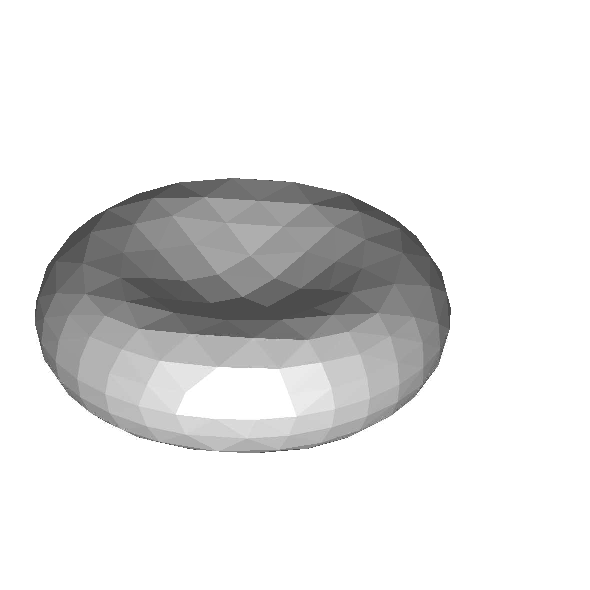
\includegraphics[width=7.5cm]{img/RBC512.pdf}\label{fig:rbc512}}\qquad
	\subfloat[][2048 panels]{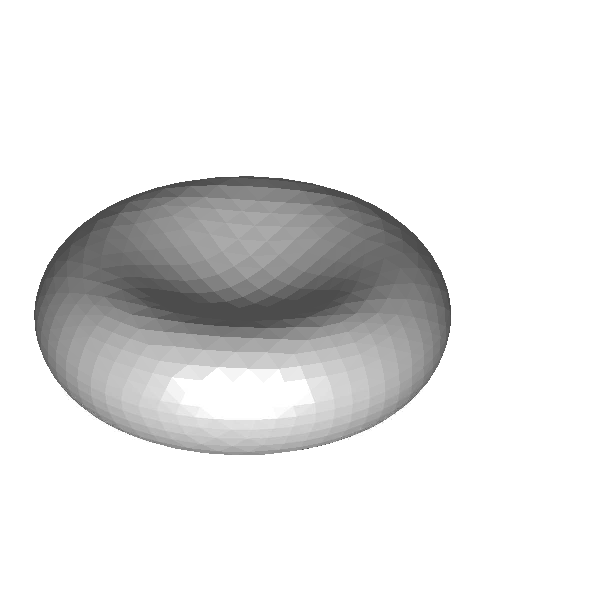
\includegraphics[width=7.5cm]{img/RBC2048.pdf}\label{fig:rbc2048}}\qquad
	\caption{Triangular discretizations of an ethrocyte, parameterized from a sphere.}
	\label{fig:glob_rbc}
\end{figure}
\end{center}

When placed in a flow with $U_x = 1,\; \mu=10^{-3}$, we obtain the traction force in the $x$-direction, shown in figure \ref{fig:stokes_rbc_traction}.

\begin{figure}[h]
\begin{center}
	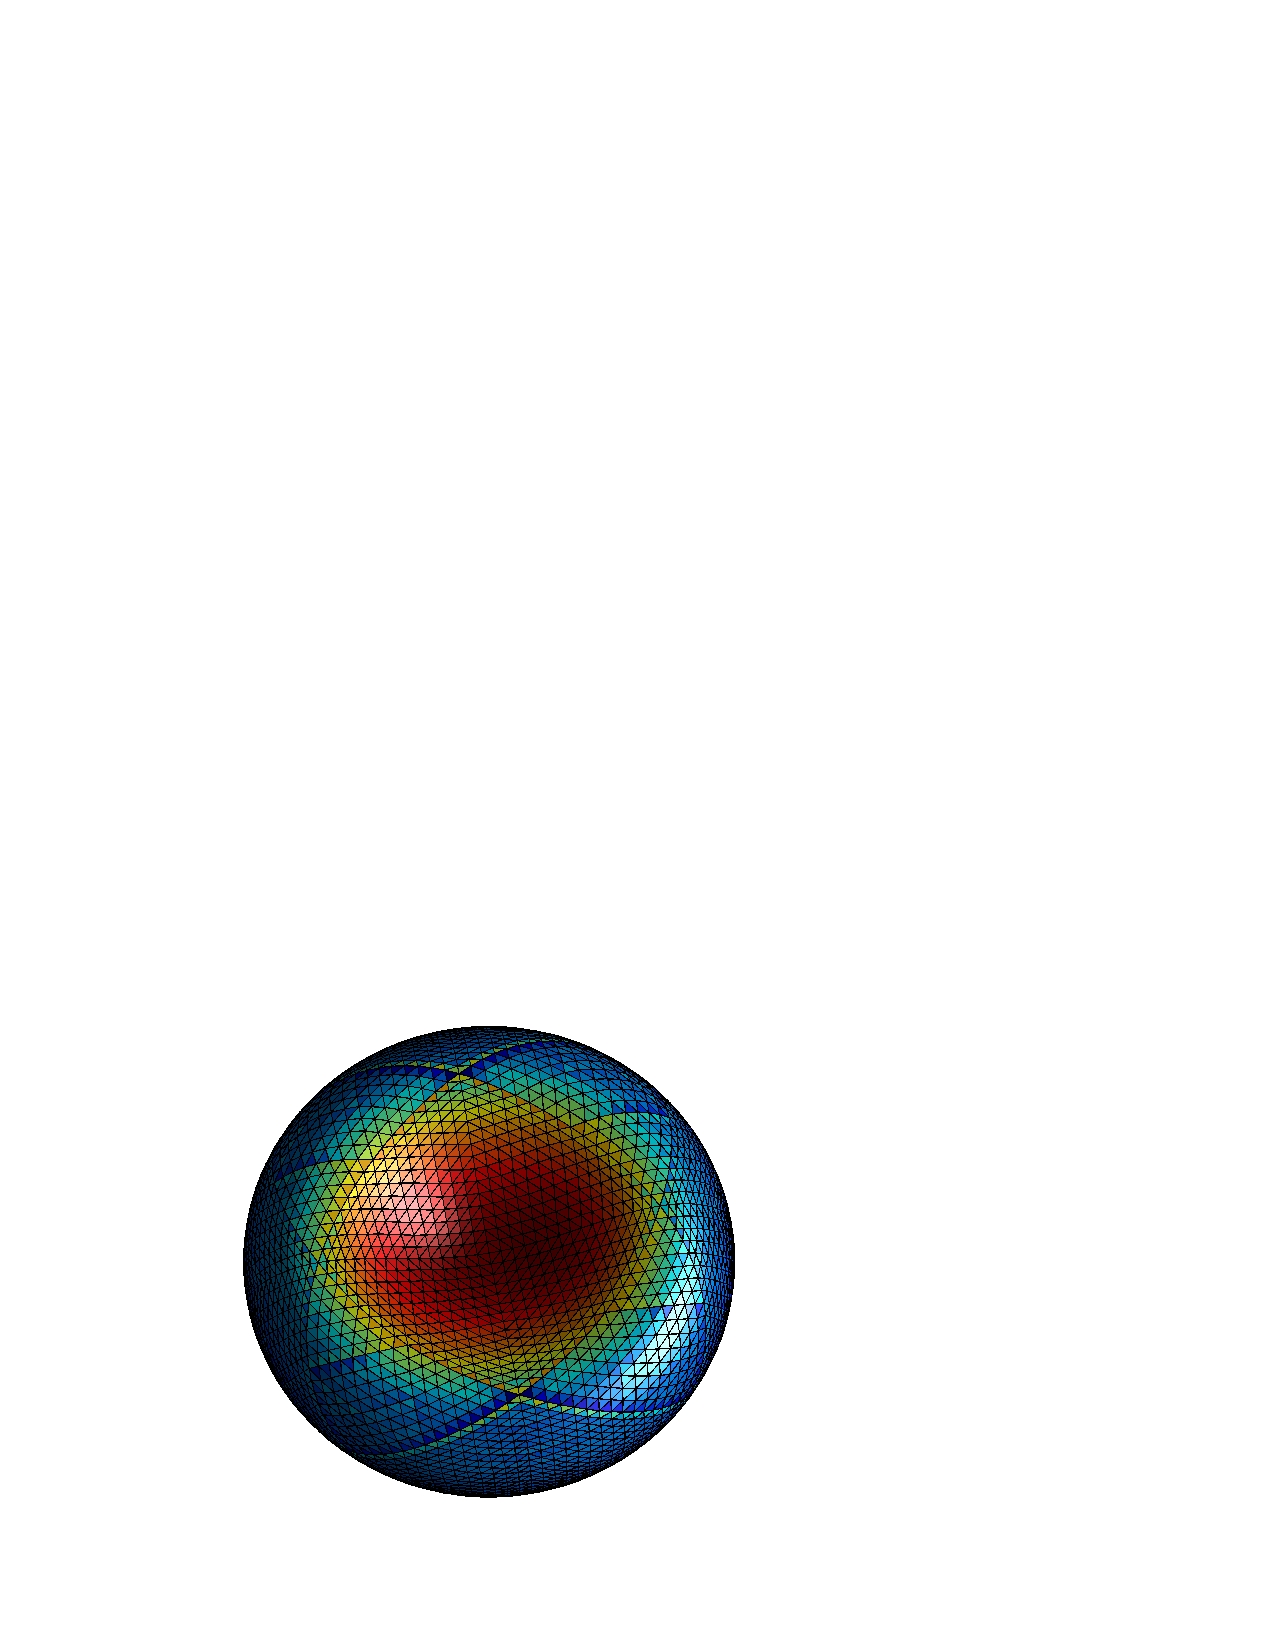
\includegraphics[width=14cm]{img/RBCTraction2.pdf}
	\caption{Traction force $t_x$ exerted in the $x$-direction on an Ethrocyte with 8192 panels, $p=16$, $\pmin=5$ solved to $10^{-5}$ tolerance}
	\label{fig:stokes_rbc_traction}
\end{center}
\end{figure}

While we do not have any kind of analytic expression for any of the flow quantities, we can still test the correctness of our method by checking if our calculated results converge as expected to some extrapolated value. As we tested the convergence of the drag force for convergence purposes with the sphere, it is a natural choice to use it for the ethrocyte as well. To obtain an extrapolated value for the drag, we use Richardson extrapolation \cite{roache1998}, choosing the calculated drag force from $3$ different meshes, with a constant refinement factor, $C$ (in this case $4$). Then, to calculate the extrapolated force value, $\bar{f}$, we  use the formula below, with $f_1$ being the coarsest mesh, and $f_3$ the finest.

\begin{equation}
	\bar{f} = \frac{f_1f_3-f_2^{2}}{f-1 -2f_2+f_3}
\end{equation}

Another useful quantity we obtain from this procedure, is the \emph{observed order of convergence}, a measure of the true convergence obtained with our method. Denoted by $p$, this is given by

\begin{equation}
	p = \frac{\ln{\left(\frac{f_2-f_1}{f_3-f_2}\right)}}{\ln{C}}.
\end{equation}

Using the mesh, $f_x$ value pairs given in table \ref{tab:rbc_richardson_values}, we calculate the converged drag force to be $f_x = -0.0834$, and the observed order of convergence to be $0.481$. This shows both that our solution is converging spatially to a value, and that the rate of convergence is $\O{\sqrt{N}}$, the same as observed for the sphere test case.

\begin{table}[htdp]
\begin{center}
\begin{tabular}{c|c}
	$N$ & $f_x$ \\
	& \\\hline
	& \\
	$512$ & $-0.059$ \\
	& \\
	$2048$ & $-0.071$ \\ 
	& \\
	$8192$ & $-0.077$ \\
%	& \\
%	$32768$ & $-0.080$
\end{tabular}
\end{center}
\caption{Values of mesh size and calculated drag force for convergence study}
\label{tab:rbc_richardson_values}
\end{table}%

To further illustrate this important result, we can use the extrapolated $f_x$ as an ``exact value'' in order to calculate errors at each of our mesh points. This error is plotted in figure \ref{fig:rbc_extrapolated_convergence}, where the first 3 points were used to calculate the extrapolated value, and the final, largest point was used as a test.

\begin{figure}
\begin{center}
	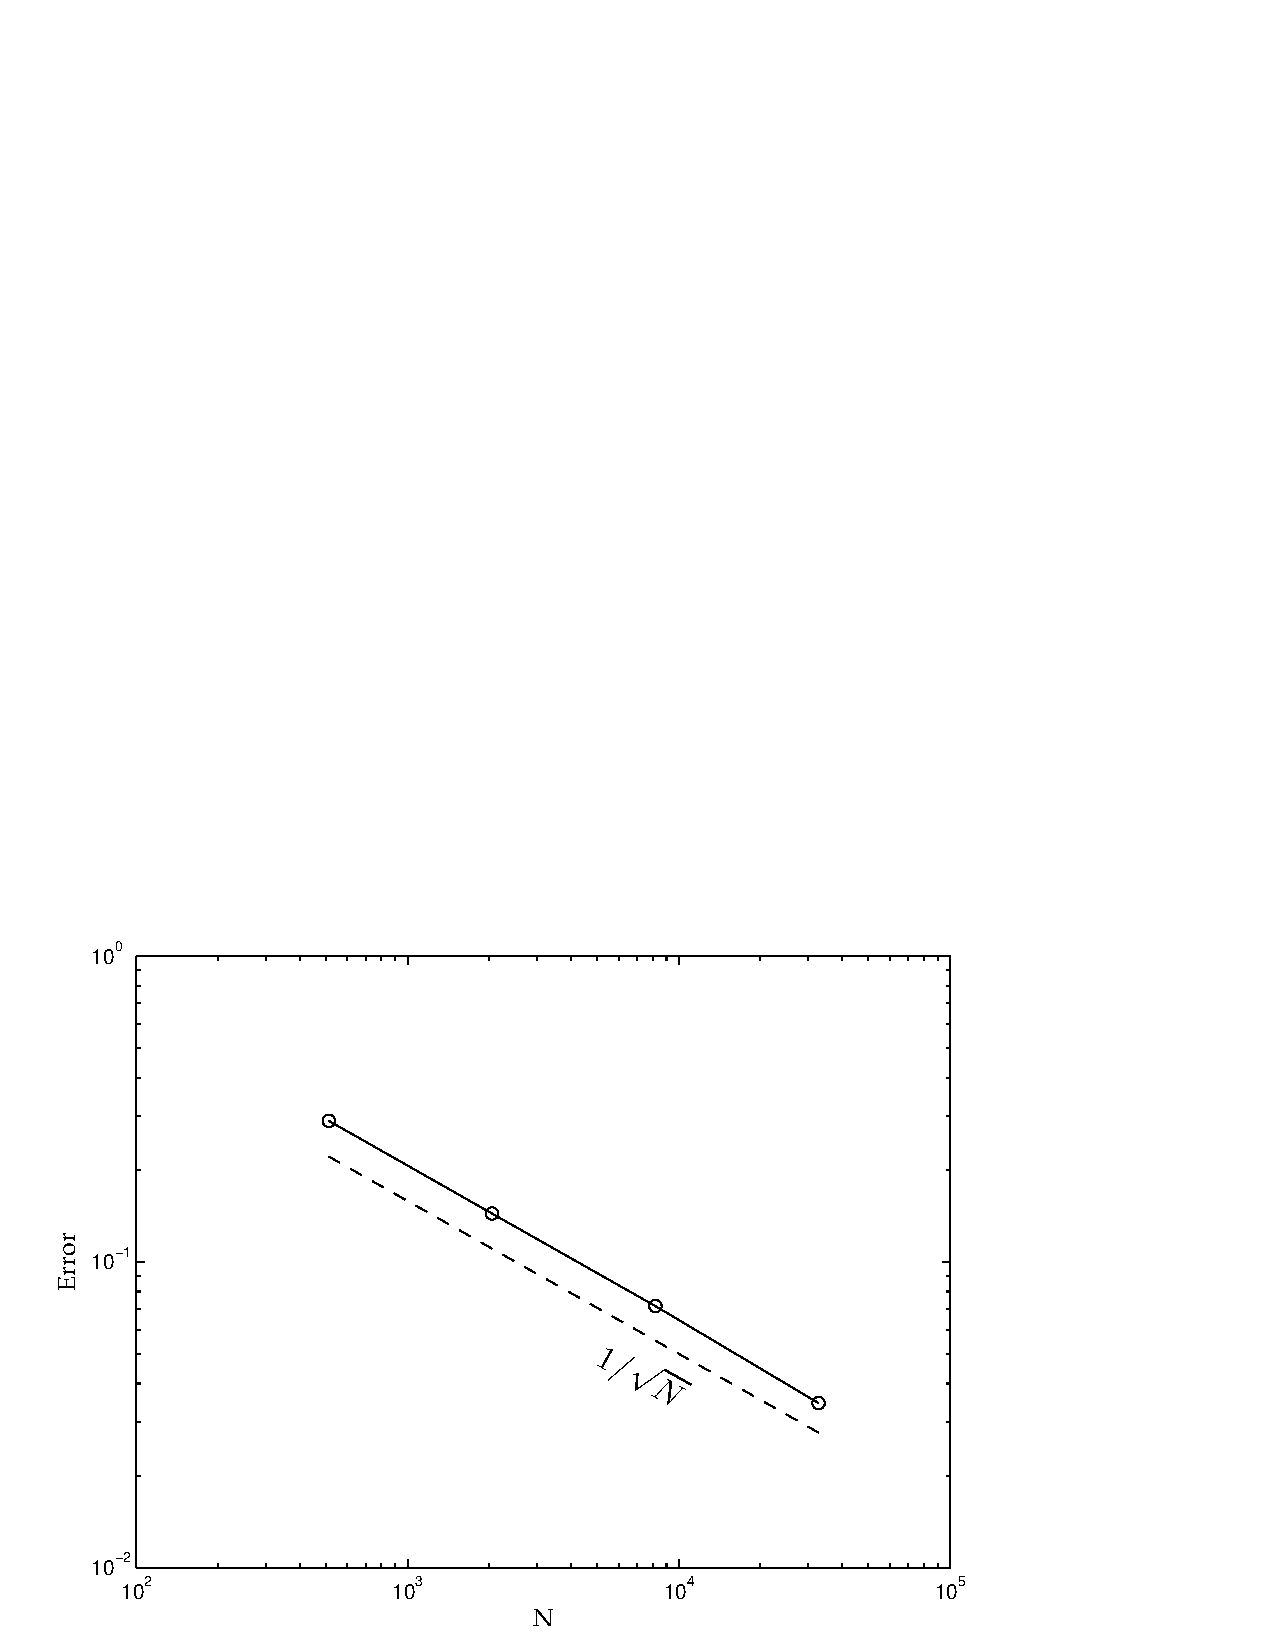
\includegraphics[width=12.5cm]{img/ExtrapolatedConverged.pdf}
	\caption{Observed convergence for Ethrocyte with respect to extrapolated value}
	\label{fig:rbc_extrapolated_convergence}
\end{center}
\end{figure}

This result shows that we are observing the same order or convergence for the ethrocyte case as for the simpler sphere --- this gives us more confidence that our {\fmmbem} solver is behaving as expected.

%%%%%%%%%%%%%%%%%%%%%%%%%%%%%%%%%%%%%%%%%%%%%%%
%%%%%% MULTIPLE CELLS
%%%%%%%%%%%%%%%%%%%%%%%%%%%%%%%%%%%%%%%%%%%%%%%
\section{Multiple Cells}\label{sec:multiple_cells}

While the flow around a single ethrocyte is more interesting than flow over a sphere, it is still not of much interest. For a more substantial problem, we look at multiple ethrocytes together, representing a single instant of blood flow in an artery / vein.

Due to the nature of the {\bem} formulation, the only difference between a single ethrocyte and multiple ones, is that the total number of panels is going to increase, and if we were to be using a dense matrix instead of the {\fmm}, it would increase in size from $(3N)\times (3N)$ to $(3N_cN)\times (3N_cN)$, where $N_c$ is the number of cells we choose to use. In the {\fmm} case, we simply have more source and target panels, and due to the $\O{N}$ scaling, the time taken for each matrix-vector product should increase linearly.

In order to generate an interesting combination of cells, we repeatedly take a single ethrocyte, then apply a random rotation and shift in space, ensuring that cells do not overlap. An example of this is shown in figure \ref{fig:multiple_cells}.

\begin{figure}
\begin{center}
	% do this image horizontally
	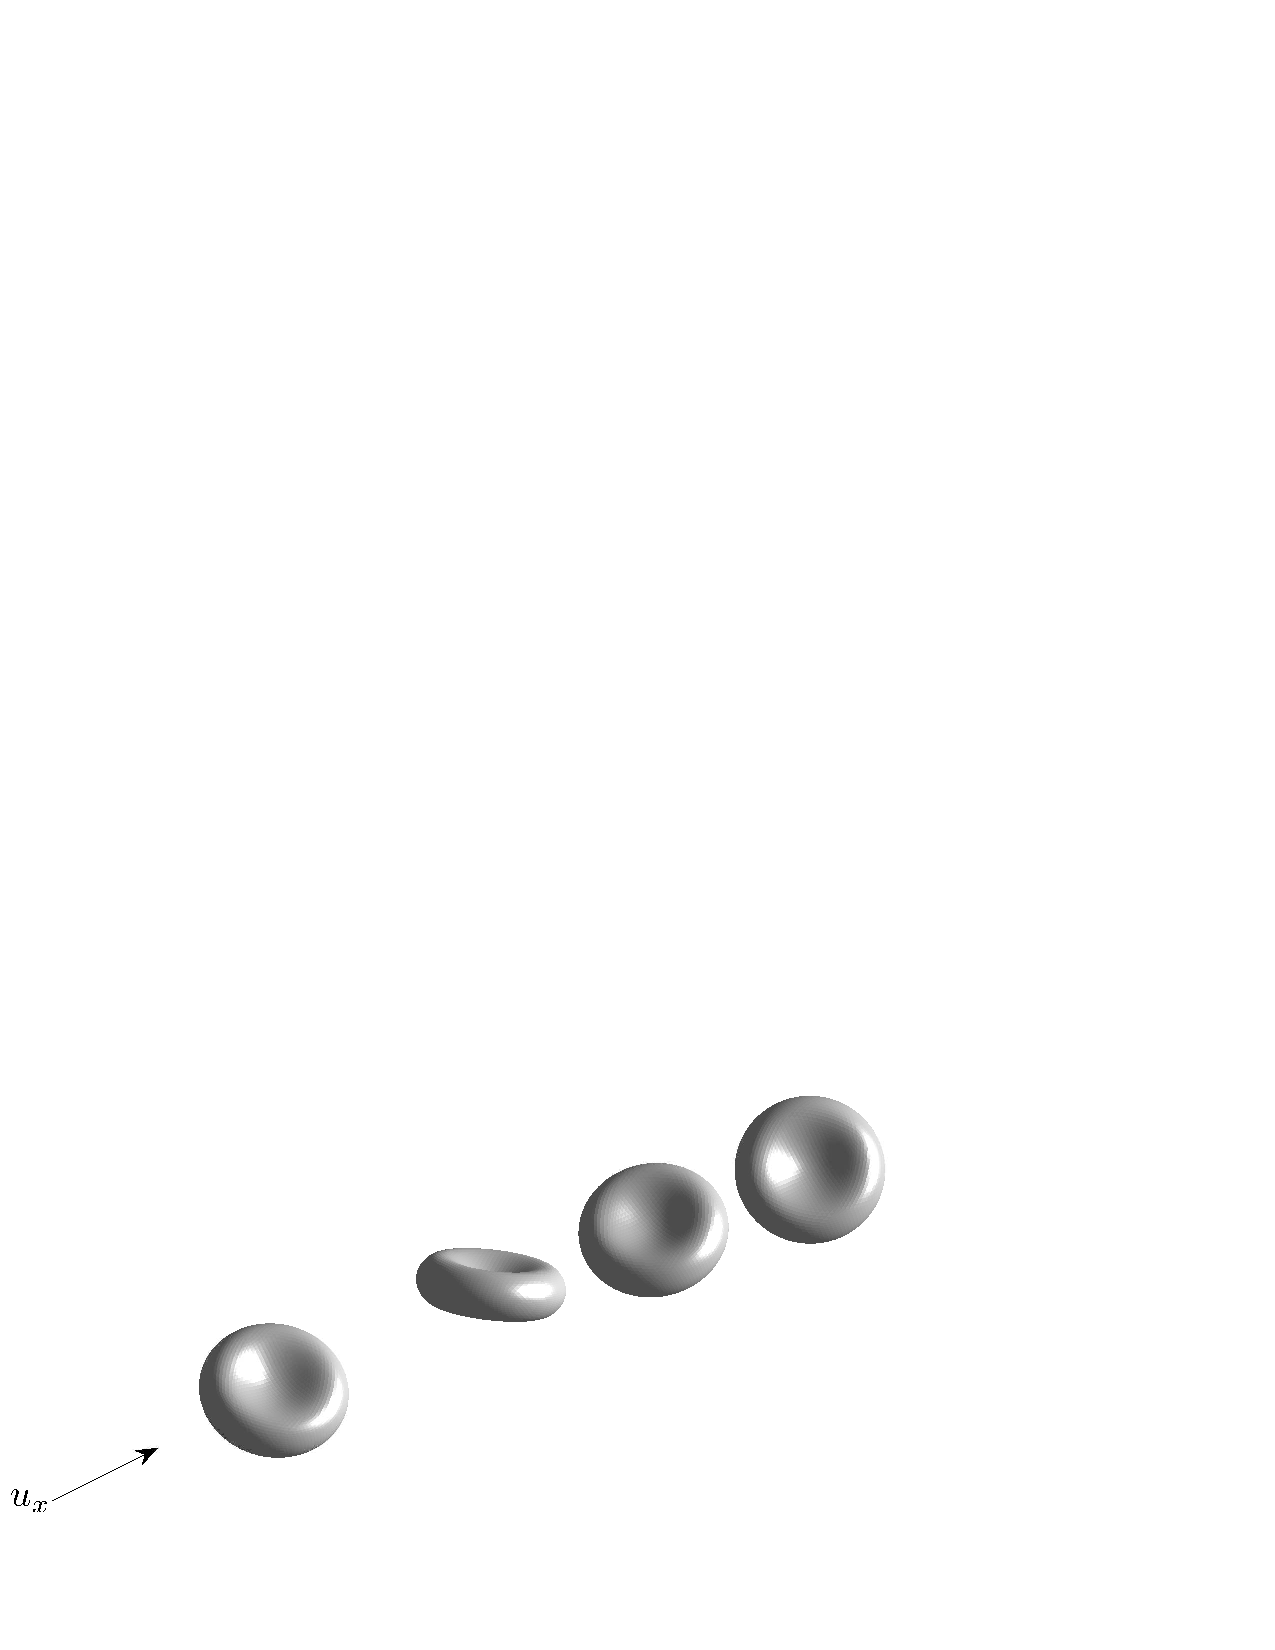
\includegraphics[width=14cm]{img/4Cells_arrow.pdf}
	\caption{Example surfaces for 4 Ethrocytes in fluid}
	\label{fig:multiple_cells}
\end{center}
\end{figure}

Given our ability to generate geometries with arbitrary numbers of cells, we can perform a number of interesting experiments. First, we study the properties of the resulting linear system (conditioning of the system), especially how the number of iterations changes as we increase $N_c$. Next, we examine the benefits of both preconditioners and relaxation (and combinations of both) on a non-trivial problem.

%%%%%%%%%%%%%%%%%%%%%%%%%%%%%%%%%%%%%%%%%%%%%%%
%%%%%% CONVERGENCE PROPERTIES
%%%%%%%%%%%%%%%%%%%%%%%%%%%%%%%%%%%%%%%%%%%%%%%
\subsection{Convergence Properties}\label{sec:convergence_properties}

As we move from a single ethrocyte to many, we might suspect that the resulting linear system would become increasingly harder to solve. This can result from the fact that the system has increased in size by a factor of the number of cells, or from the natural assumption that as we add cells that are disconnected from each other, it becomes tougher to solve the system.

We would prefer to investigate this topic by calculating the condition number of actual problems, but for problem sizes that would be interesting ($8192$ panels / cell), the amount of memory required to calculate the condition would be very large. For instance, the aforementioned $8192$ panel case gives a dense matrix with $6\times 10^{8}$ entries, taking $4.6\text{GB}$ in double precision. Raising the number of panels to 32768, we have $9.7\times10^{9}$ entries in our matrix, taking $73.7\text{GB}$ in double precision, a prohibitive amount. 

While there has been some theoretical work on the condition number of matrices arising from 2D {\bem} problems, \cite{DijkstraMattheij06,dijkstramattheij2007}, and some numerical notes involving condition numbers for 3D MEMS problems (Stokes) \cite{frangi2005}, there are no analytical formulations to approximate the condition number for 3D Stokes, and the problems we are interested in are too large to produce a dense matrix representation and directly obtain the condition number. Due to these restrictions, we choose to approach this problem in terms of problem size and the number of iterations required to obtain a solution with a desired residual, using the iteration count as a proxy to the condition number.

First, as a baseline, we will look at the iterations required to solve the system for a single ethrocyte, whilst refining the surface mesh.

\begin{figure}
\begin{center}
	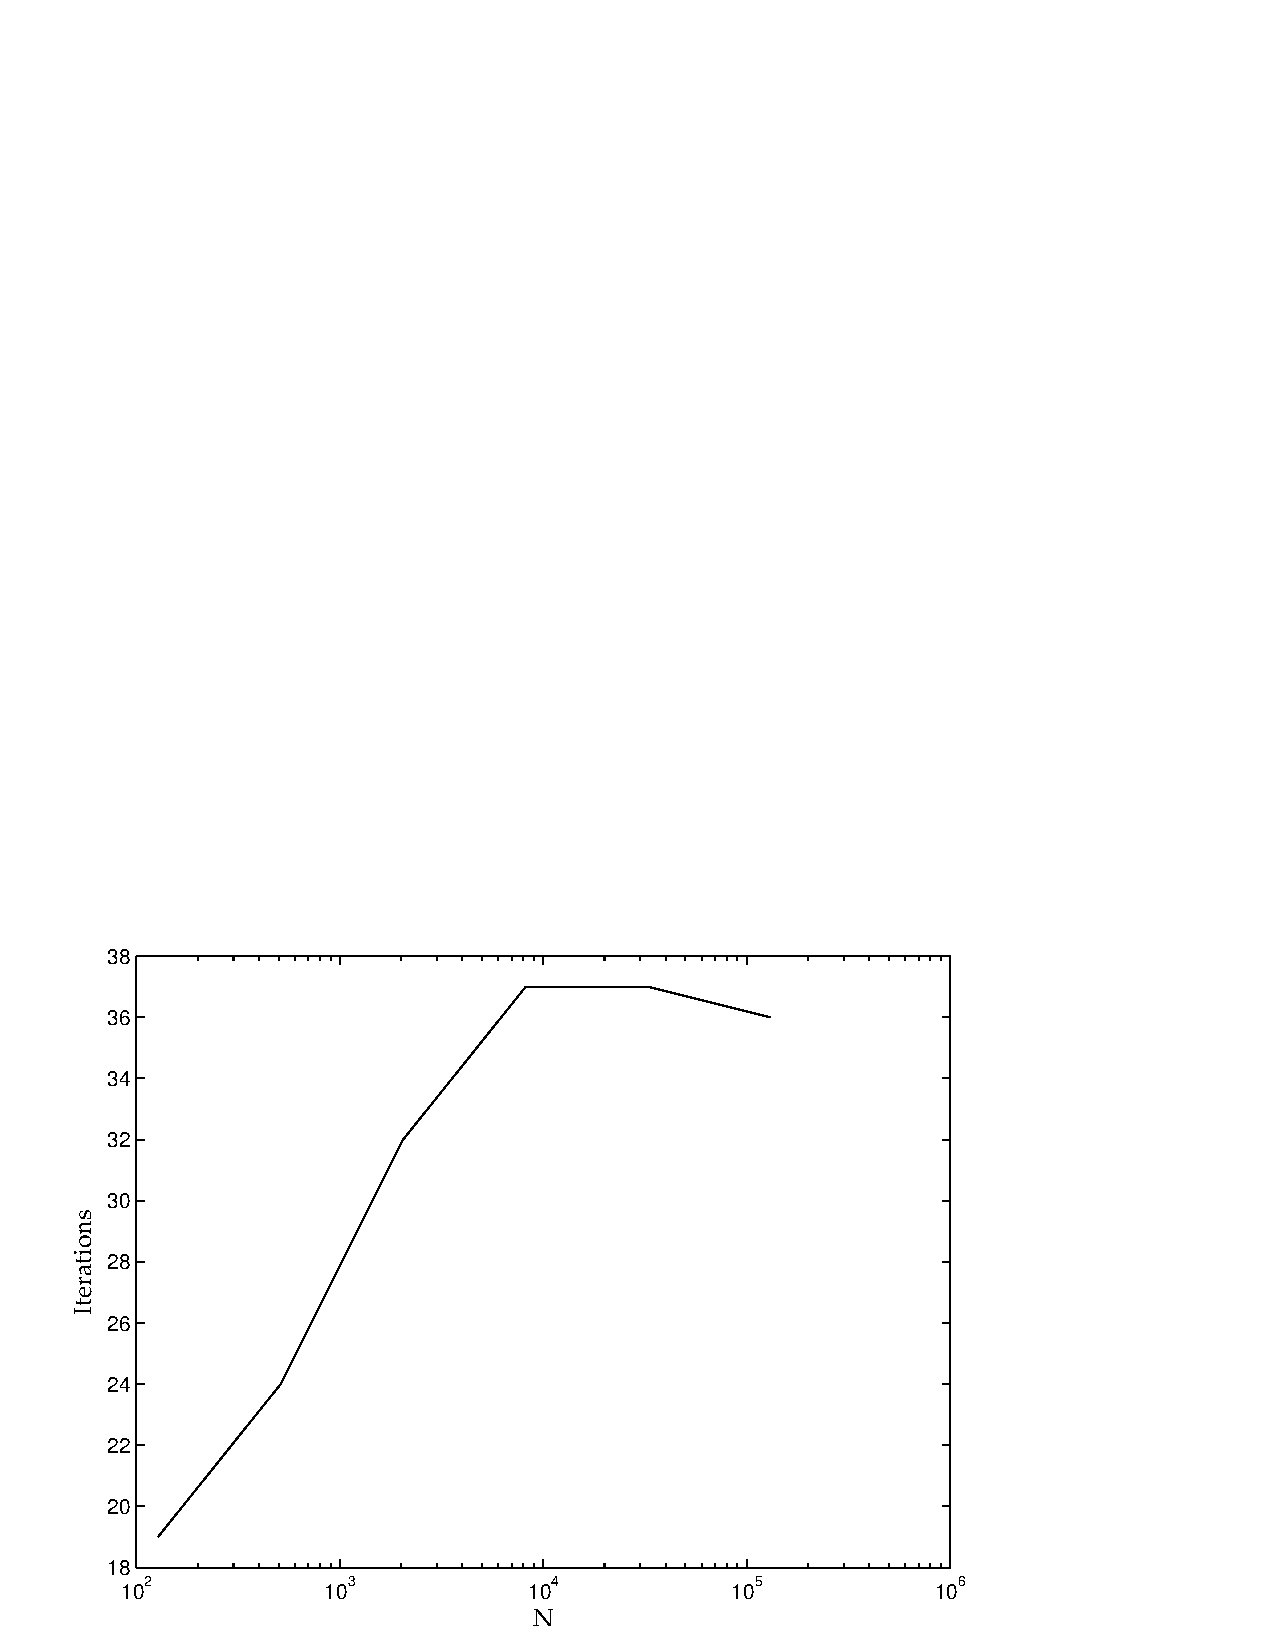
\includegraphics[width=12cm]{img/StokesSingleCellIterations.pdf}
	\caption{Iterations for Ethrocyte system to converge. $p = 16$, desired residual $10^{-5}$}
	\label{fig:single_cell_iterations}
\end{center}
\end{figure}

In figure \ref{fig:single_cell_iterations} we can see that as we increase from $128$ panels to $8192$, the number of iterations needed increases from $19$ to $37$, while as we further refine the mesh up to $131,072$ panels we see the number of iterations flatten out. This implies that beyond a certain point, the condition number of our matrix stops increasing, although without being able to test a larger system, we cannot confirm this. % [[[ IS THIS ACTUALLY TRUE??? ]]].

Now that we know how the convergence behaviour changes with respect to the number of panels per ethrocyte, we can look at how it changes with respect to multiple cells. We take advantage of the nature of our geometry creation (that is, the refinement factor is 4) to both test how the convergence changes as we increase the number of cells, as well as the effect of the number of panels per cell. In all cases $p = 16,\;p_{\text{min}} = 5$ and the solver tolerance is set to $10^{-5}$.

\begin{figure}
\begin{center}
	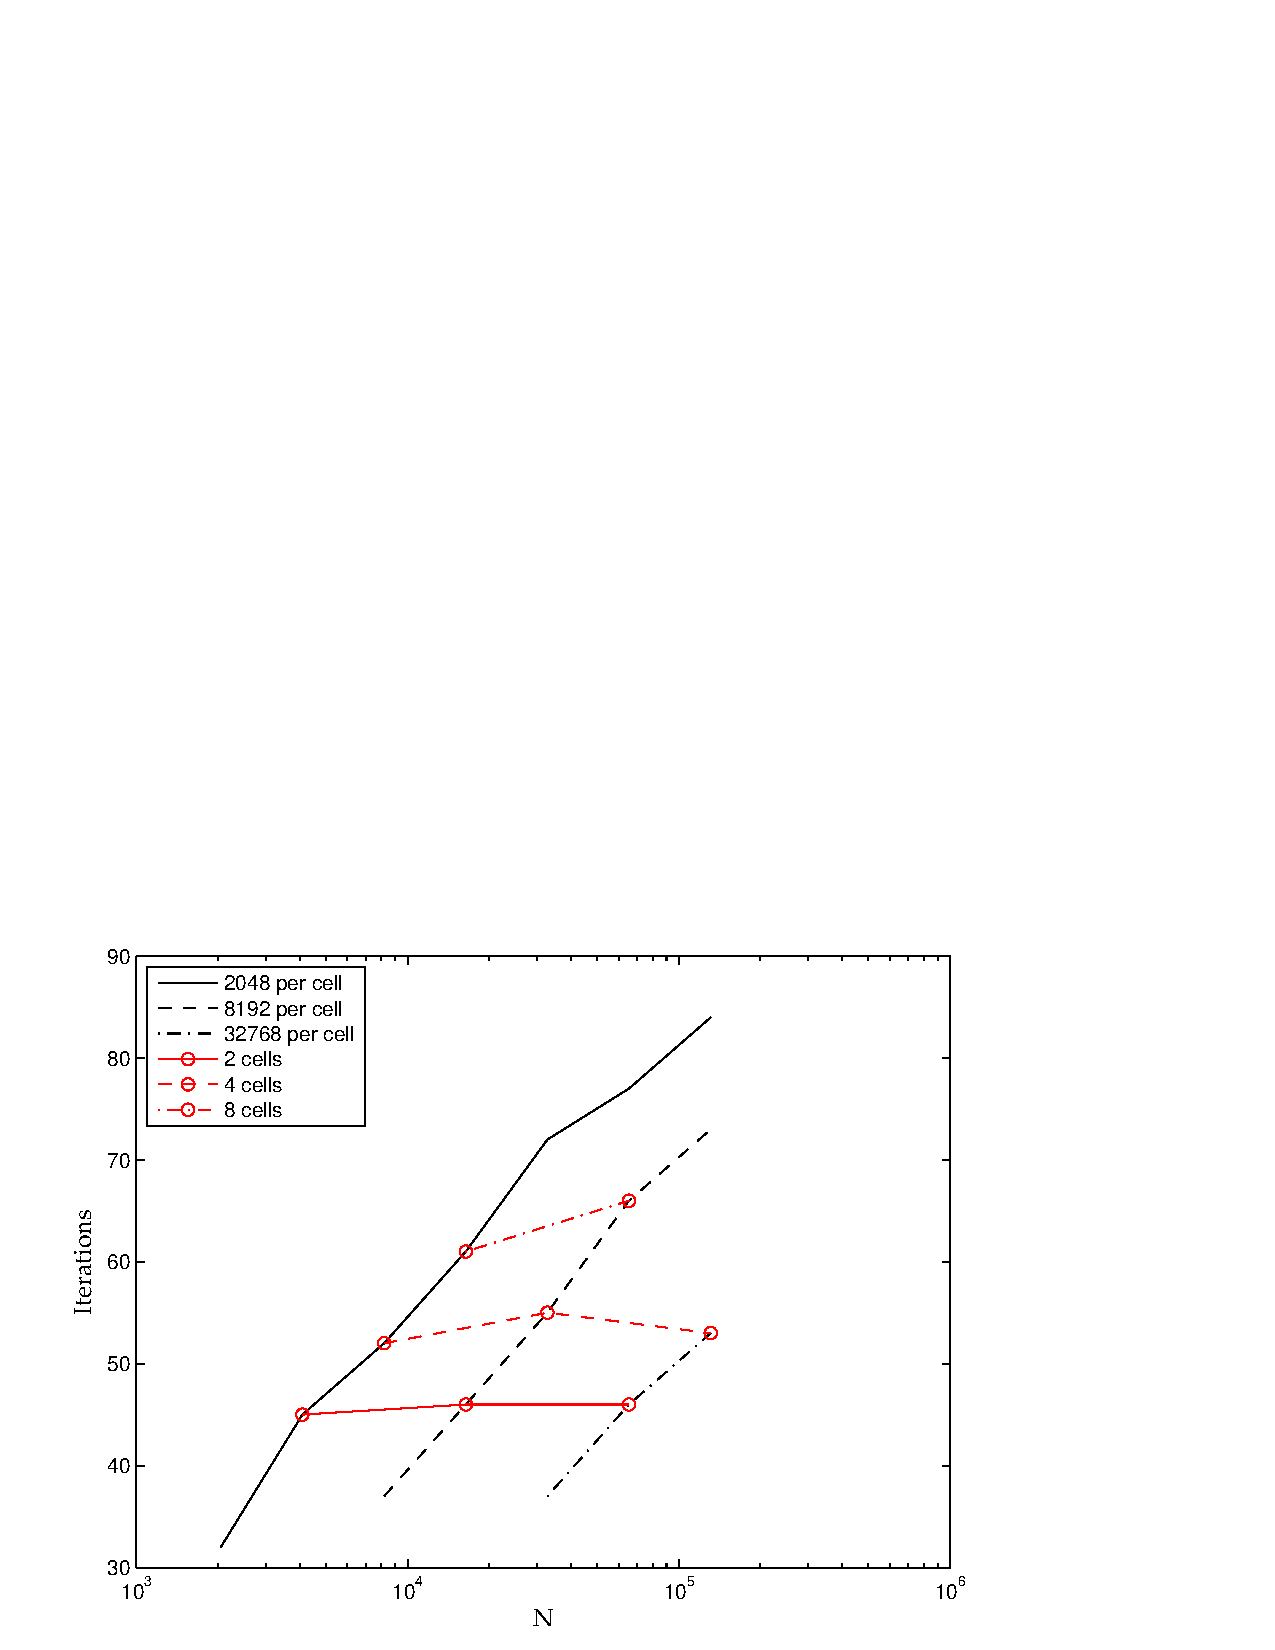
\includegraphics[width=11.5cm]{img/StokesMultipleCellsIterations.pdf}
	\caption{Iterations for system from multiple Ethrocyte to converge. $p = 16$, desired residual $10^{-5}$}
	\label{fig:multiple_cell_iterations}
\end{center}
\end{figure}

Figure \ref{fig:multiple_cell_iterations} shows how the number of iterations needed to converge changes with respect to the number of cells used and with respect to the number of panels per cell. In all 3 cases, $2048,\;8192$ or $32768$ panels per cell, we see a sharp increase in the number of iterations as the number of cells increases. Interestingly, if we look at the number of iterations required for a set number of cells, they are very similar for each case -- it makes little difference how many panels comprise each cell, the convergence properties are dominated by the number of cells. For instance, the system for 2 cells takes 45, 46 and 46 iterations for 2048, 8192 and 32768 panels per cell. Similarly, for 4 cells, 52, 55 and 53 iterations were needed for the analogous cases.

This is encouraging for the use of relaxation, as state-of-the-art simulations often involve 40 or more ethrocytes \cite{Liu2009,RahimianETal2010}, implying that we are likely to require a large number of iterations, potentially $\O{100}$, giving large potential gains in speed.

%%%%%%%%%%%%%%%%%%%%%%%%%%%%%%%%%%%%%%%%%%%%%%%
%%%%%% RELAXATION
%%%%%%%%%%%%%%%%%%%%%%%%%%%%%%%%%%%%%%%%%%%%%%%
\subsection{Relaxation}\label{sec:stokes_ethrocyte_relaxation}

Now that we have established the convergence properties of systems involving ethrocytes, we start to look at the advantages of using a relaxation scheme. With the results shown in figures \ref{fig:single_cell_iterations} and \ref{fig:multiple_cell_iterations}, we expect a large number of iterations to be needed in all cases. In addition to this, from figure \ref{fig:stokes_relaxation_breakdown} in our experiments on a spherical object, we expect to spend large numbers of iterations at a smaller value of $p$. Finally, figure \ref{fig:stokes_relaxation_breakdown}, shows the decrease in time for the far-field calculation when we reach our minimum $p$.

Combining these 3 observations, we can expect savings from applying a relaxation scheme for a single ethrocyte, with the gains increasing as a function of the number of cells. In all comparisons, the best parameters will be used -- for non-relaxed runs the near and far-field evaluations will be as balanced as possible, while for relaxed tests parameters will be chosen to give the shortest runtime. In every case we only look at the time taken in the solution phase (within the {\gmres} solver) as the setup (including generating the right-hand-side of the linear system) is 1) amortized over the total run, and 2) always performed at high-precision, so the behavior is identical for relaxed and fixed-$p$ cases. Small problems will not be tested, as the fastest solution will also be using a direct method, which inherently cannot use relaxation.

All experiments were performed with the settings described in table \ref{tab:cells_relaxation_settings}.

\begin{table}[h]
\begin{center}
\begin{tabular}{c|c}
 Variable & Setting \\ 
 & \\ \hline
 & \\
 $p_{\text{initial}}$ & $16$ \\
 & \\
 $p_{\text{min}}$ &  $5$ \\
 & \\
 solver tolerance & $10^{-5}$ \\
 & \\
 Near-field & Sparse matrix \\
 & \\
 Threads & $4$ \\
 & \\
 Solver & {\gmres} \\ 
 & \\
 Preconditioner & None
 
\end{tabular}
\end{center}
\caption{Ethrocyte relaxation test settings}
\label{tab:cells_relaxation_settings}
\end{table}%

Looking at the results in \ref{tab:single_cell_relaxation_results}, we see that we obtain a consistent $3-4\times$ speedup over non-relaxed results. The outlying result for $131072$ panels is due to being unable to use the significantly faster sparse-matrix representation of the near field. The variation in the other speedup numbers is a natural result of the behaviour of the {\fmm} when we choose different values of $\ncrit$ (and generate different octrees).

These results backup our original assumption that due to the combination of high numbers of iterations largely spent at low values of $p$, and the large savings from using that low $p$, we should see large time savings. Combining this observation with the known significant increase in iterations for the multiple ethrocyte case (\ref{fig:multiple_cell_iterations}), we expect to see time savings of a similar, if not greater degree.

\begin{table}[htdp]
\begin{center}
\begin{tabular}{c|c|c|c|c|c|c}

 & & \multicolumn{2}{c|}{Non-relaxed} & \multicolumn{2}{c|}{Relaxed} \\
 & & \multicolumn{2}{c|}{} & \multicolumn{2}{c|}{} \\
 N & \# unknowns & $\ncrit$ & $t_{\text{solve}}$ & $\ncrit$ & $t_{\text{solve}}$ & Speedup \\
 & & & & & \\ \hline
 & & & & & \\
 2048 & 6144 & 200 & 44.5 & 100 & 11.0 & 4.05 \\
 & & & & & \\
 8192 & 24576 & 400 & 177 & 150 & 52.4 & 3.37 \\
 & & & & & \\
 32768 & 98304 & 400 & 848 & 150 & 223 & 3.80 \\
 & & & & & \\
 131072 & 393216 & 600 & 6386\footnotemark[1] & 150 & 874 & 7.31\footnotemark[1] \\
 & & & & & \\
	
\end{tabular}
\end{center}
\caption{Single Ethrocyte relaxation test results, performed with initial $p=16$, $\pmin=5$, solved to $10^{-5}$ tolerance.}
\label{tab:single_cell_relaxation_results}
\end{table}%

\footnotetext[1]{Due to memory restrictions, the sparse-matrix representation of the near-field could not be used, resulting in a much slower {\ptop} evaluation}

%\begin{landscape}
%\begin{table}[htdp]
%\begin{center}
%\begin{tabular}{c|cccccc|cccccc|cccccc|}
%
%& \multicolumn{6}{c}{2048 panels / cell} & \multicolumn{6}{c}{8192 panels / cell} & \multicolumn{6}{c}{32768 panels / cell} \\
%& & \multicolumn{2}{c}{Non-relaxed} & \multicolumn{2}{c}{Relaxed} & & & \multicolumn{2}{c}{Non-relaxed} & \multicolumn{2}{c}{Relaxed} & & & \multicolumn{2}{c}{Non-relaxed} & \multicolumn{2}{c}{Relaxed} & \\
%N & $N_c$ & $\ncrit$ & $\tsolve$ & $\ncrit$ & $\tsolve$ & speedup & $N_c$ & $\ncrit$ & $\tsolve$ & $\ncrit$ & $\tsolve$ & speedup & $N_c$ & $\ncrit$ & $\tsolve$ & $\ncrit$ & $\tsolve$ & speedup \\ \hline
%& & & & & & & & & & & & & & & & & & \\
%2048 & 1 & 200 & 44.5 & 100 & 11.0 & 4.05 & \multicolumn{6}{c}{---} & \multicolumn{6}{c}{---} \\ 
%& & & & & & & & & & & & & & & & & & \\
%8192 & 4 & 200 & 236 & 150 & 59.8 & 3.95 & 1 & 400 & 177 & 150 & 52.4 & 3.37 & \multicolumn{6}{c}{---} \\
%& & & & & & & & & & & & & & & & & & \\
%32768 & 16 & 400 & 1261 & 150 & 331 & 3.81 & 4 & 400 & 1375 & 150 & 315 & 4.37 & 1 & 400 & 848 & 150 & 223 & 3.80 \\
%& & & & & & & & & & & & & & & & & & \\
%131072 & 64 & - & - & 100 & 1606 & - & 16 & - & - & 100 & 1681 & - & 4 & - & - & - & - & - \\
%
%	
%\end{tabular}
%\end{center}
%\caption{Multiple Ethrocyte relaxation test results}
%\label{tab:multiple_cell_relaxation_results}
%\end{table}
%\end{landscape}

\begin{table}[htdp]
\begin{center}
\begin{tabular}{c|c|c|cc|cc|c}

\multicolumn{8}{c}{2048 panels / cell} \\
& & & \multicolumn{2}{c}{Non-relaxed} & \multicolumn{2}{c}{Relaxed}\\
N & \# unknowns & $N_c$ & $\ncrit$ & $\tsolve$ & $\ncrit$ & $\tsolve$ & Speedup \\ \hline
& & & & & & &  \\
2048 & 6144 & 1 & 200 & 44.5 & 100 & 11.0 & 4.05 \\ 
& & & & & & &  \\
8192 & 24576 & 4 & 200 & 236 & 150 & 59.8 & 3.95 \\ 
& & & & & & &  \\
32768 & 98304 & 16 & 400 & 1261 & 150 & 331 & 3.81 \\
& & & & & & &  \\
131072 & 393216 & 64 & 300 & 9982\footnotemark[1] & 100 & 1606 & 6.22\footnotemark[1] \\

\end{tabular}
\end{center}
\caption{Multiple Ethrocyte relaxation test results 2048 panels / cell}
\label{tab:multiple_cell_relaxation_results_2048}
\end{table}

%\footnotetext[2]{Sparse matrix form for near-field was unable to be used in this case for memory reasons}

\begin{table}[htdp]
\begin{center}
\begin{tabular}{c|c|c|cc|cc|c}

\multicolumn{8}{c}{8192 panels / cell} \\
& & &  \multicolumn{2}{c}{Non-relaxed} & \multicolumn{2}{c}{Relaxed}\\
N & \# unknowns & $N_c$ & $\ncrit$ & $\tsolve$ & $\ncrit$ & $\tsolve$ & speedup \\ \hline
& & & & & & &  \\
8192 & 24576 & 1 & 400 & 177 & 150 & 52.4 & 3.37 \\ 
& & & & & & &  \\
32768 & 98304 & 4 & 400 & 1375 & 150 & 315 & 4.37 \\
& & & & & & &  \\
131072 & 393216 & 16 & 300 & 15980\footnotemark[1] & 100 & 1692 & 9.44\footnotemark[1] \\

\end{tabular}
\end{center}
\caption{Multiple Ethrocyte relaxation test results for 8192 panels / cell}
\label{tab:multiple_cell_relaxation_results_8192}
\end{table}

\begin{table}[htdp]
\begin{center}
\begin{tabular}{c|c|c|cc|cc|c}

\multicolumn{8}{c}{32768 panels / cell} \\
& & & \multicolumn{2}{c}{Non-relaxed} & \multicolumn{2}{c}{Relaxed}\\
N & \# unknowns & $N_c$ & $\ncrit$ & $\tsolve$ & $\ncrit$ & $\tsolve$ & speedup \\ \hline
& & & & & & &  \\
32768 & 98304 & 1 & 400 & 848 & 150 & 223 & 3.80 \\
& & & & & & &  \\
131072 & 393216 & 4 & 300 & 9629\footnotemark[1] & 100 & 1247 & 7.72\footnotemark[1] \\	
\end{tabular}
\end{center}
\caption{Multiple Ethrocyte relaxation test results for 32768 panels / cell}
\label{tab:multiple_cell_relaxation_results_32768}
\end{table}

\begin{figure}[h]
\begin{center}
	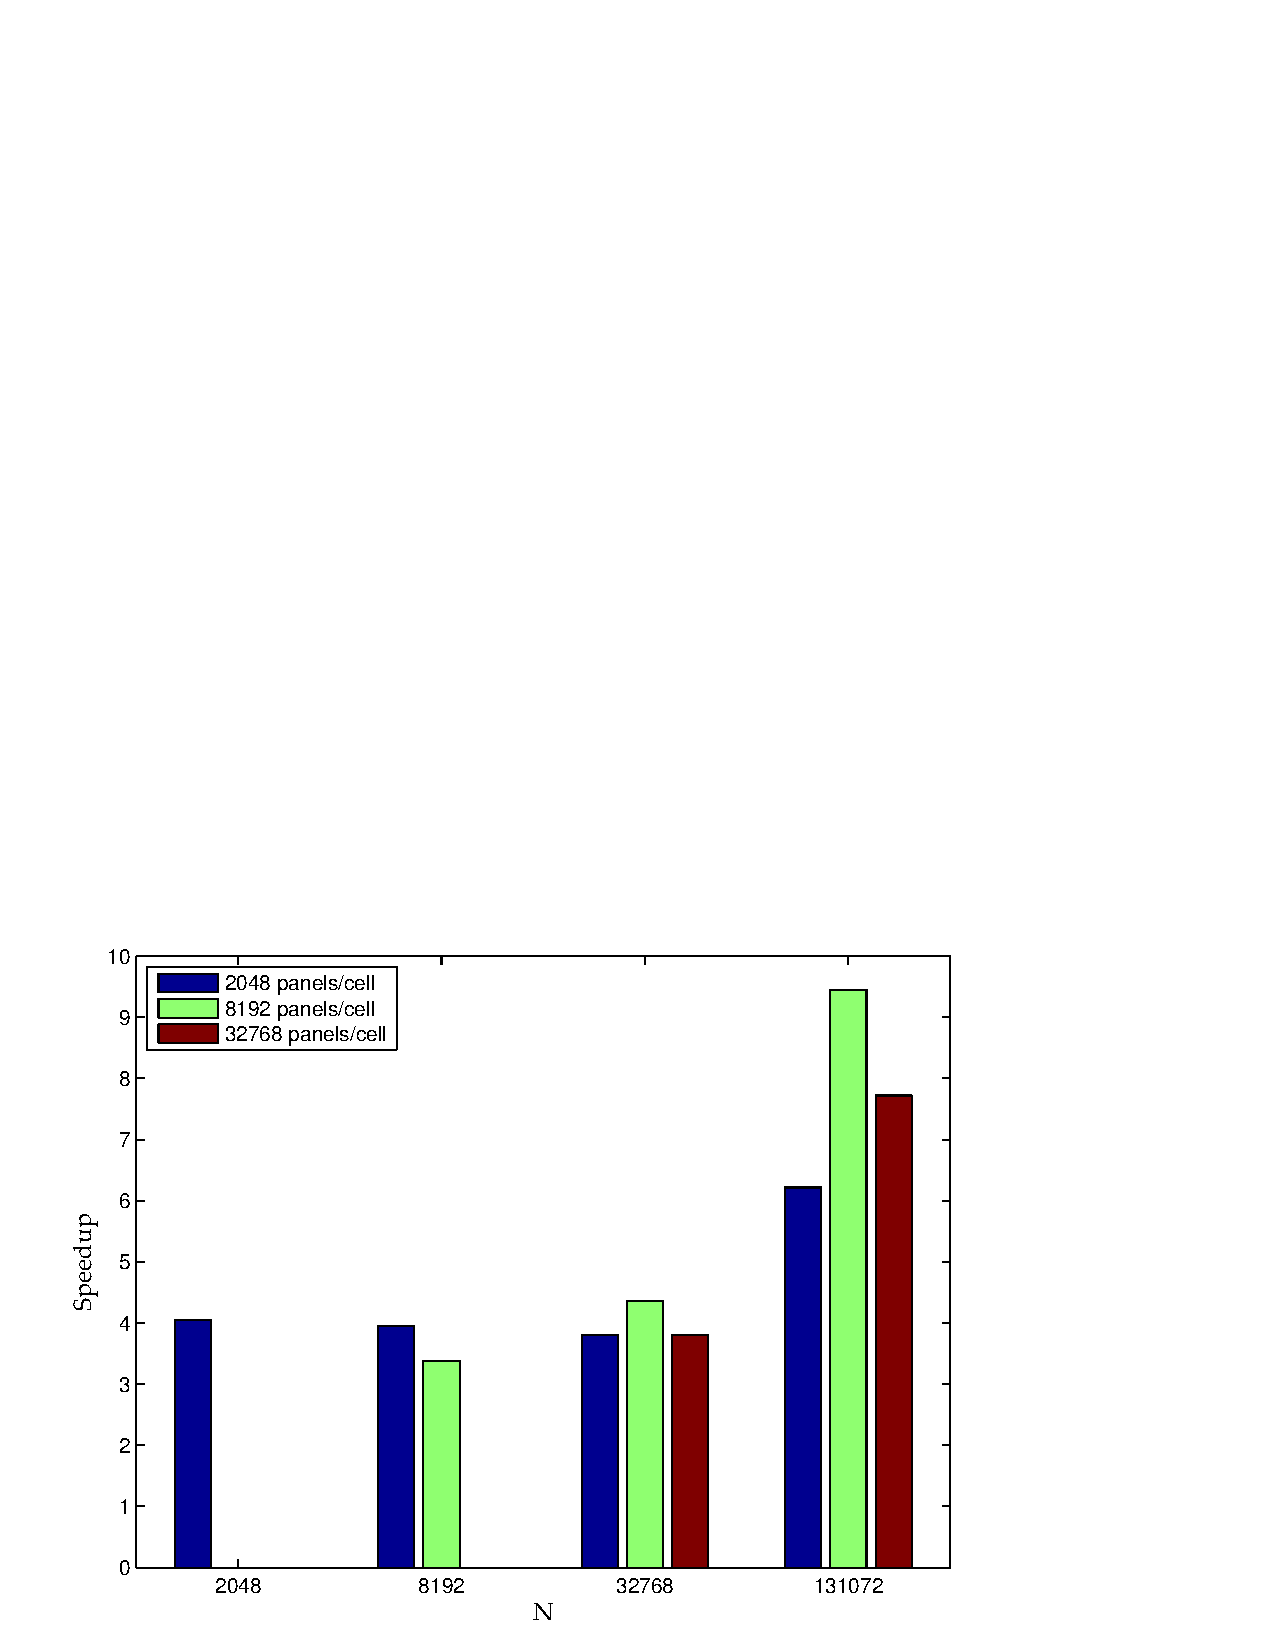
\includegraphics[width=14cm]{img/StokesMultipleCellsSpeedup.pdf}
	\caption{Speedups from multiple ethrocyte tests with varying panels / cell and number of cells. $p = 16$, desired residual $10^{-5}$}
	\label{fig:multiple_cell_speedup}
\end{center}
\end{figure}

Tables \ref{tab:multiple_cell_relaxation_results_2048}-\ref{tab:multiple_cell_relaxation_results_32768} present timing results for both relaxed and non-relaxed solvers for systems involving multiple ethrocytes. The results are also summarized in figure \ref{fig:multiple_cell_speedup}. The first result to note is that the smallest speedup obtained was $3.37\times$, for a single cell of 8192 panels. This shows that even for a relatively small test problem, the speedup due to relaxation is large. Second, for tests where both solvers could utilize the sparse near-field representation, the average speedup is $3.89\times$, a major gain. Finally, we see again that for large problems the memory efficiency of the lower $\ncrit$ for relaxed solves is vital, as for these cases the speedup jumps to between $6-9\times$.

All of these multiple ethrocyte results confirm our expectations from the single cell tests, that we can obtain significant and worthwhile speedups simply from the use of a relaxation scheme and modifying $\ncrit$ to maintain a reasonable balance between {\ptop} and {\mtol} over the course of an iterative solve.

%%%%%%%%%%%%%%%%%%%%%%%%%%%%%%%%%%%%%%%%%%%%%%%
%%%%%%%%%%% PREVIOUS WORK
%%%%%%%%%%%%%%%%%%%%%%%%%%%%%%%%%%%%%%%%%%%%%%%
%\subsection{Comparison with previous work}\label{sec:rbc_previous_comparison}
%
%We have now shown the advantage of relaxation within our own solver for red blood cell problems, so it will be interesting to look at some previous work solving a similar problem, and estimate the benefits that could have been gaining if they had implemented a similar relaxation scheme to ours.
%
%First, we look at the most similar work to ours, using 7500 panels per cell, and 40 cells \cite{Liu2009}. This experiment consisted of 40 cells, each of 7500 panels, giving 300k total panels and 900k degrees of freedom, roughly $2\times$ the size of problem we can currently perform. The value of $\ncrit$ and the exact formulation solved was not given. This system was solved in 730 minutes, taking 49 iterations at $p=15$, solving to a tolerance of $10^{-4}$. We can replicate the majority of these options, although for 40 cells we must use 2048 panels per cell, giving 81920 total panels. This experiment took 33 iterations to converge and 1793s for the fixed-$p$ case, and 639s for the relaxed solver, giving a speedup of $2.80\times$. This speedup is lower than those reported for our experiments due to the change in solver tolerance and thus fewer iterations.

% Other major work in the same field involves a different kind of problem -- using many, less well-resolved cells of a slightly different type, vessicles, in an attempt to simulate something resembling one or more drops of blood. In the first study in this category, $\O{1000}$ panels per cell are used in a time-dependant simulation with up to 600 cells (~600k panels, 1.8m unknowns). This run involved 4500 time steps, in circa 10 days. Remaining details, including the number of iterations required per timestep were not given. 


%%%%%%%%%%%%%%%%%%%%%%%%%%%%%%%%%%%%%%%%%%%%%%%
%%%%%%%%%%% PRECONDITIONERS
%%%%%%%%%%%%%%%%%%%%%%%%%%%%%%%%%%%%%%%%%%%%%%%
\subsection{Preconditioners}\label{sec:rbc_preconditioners}

Even with the results demonstrated in \S\ref{sec:stokes_ethrocyte_relaxation}, the traditional manner of reducing solution time is to use a preconditioner to lower the iteration count, so we must consider the following questions:

\begin{enumerate}
\item Is our relaxation scheme faster than a traditional preconditioned problem solved with fixed $p$?
\item Does our relaxation scheme benefit additionally when used in a preconditioned system?
\end{enumerate}

To find answers to these 2 queries, we perform some experiments on multiple ethrocytes, using the block-diagonal and local preconditioners described in \S\ref{subsec:preconditioners}. As an initial test, we perform a small calculation, with $4$ cells, each of $2048$ panels. This results in a total of $8192$ panels, and a linear system with $24576$ unknowns. This is sizable enough to draw some initial conclusions, yet small enough that it can be performed in $1-2$ minutes in the relaxed case (and $< 5$ minutes with the non-relaxed solver).

Table \ref{tab:relaxation_preconditioning} presents iteration counts and total solution times for both relaxed and non-relaxed solvers for preconditioned and non-preconditioned solvers. In all experiments $\ncrit = 150$ for relaxation, and $\ncrit = 400$ for non-relaxed cases.

\begin{table}[htdp]
\begin{center}
\begin{tabular}{c|c|c|c|c|c|c}

 & \multicolumn{3}{c|}{Relaxed} & \multicolumn{3}{c}{Fixed $p$} \\
 & \multicolumn{3}{c|}{} & \multicolumn{3}{c}{} \\
 Preconditioner & iterations & $\tsolve$ & speedup & iterations & $\tsolve$ & speedup\\
 & & & & & & \\ \hline
  & & & & & &  \\
 Unpreconditioned & 52 & 59.9 & -/- & 52 & 238.0 & -/- \\
 & & & & & & \\
 Block-Diagonal & 45 & 60.8 & 1.18/0.98 & 45 & 212.7 & 1.18/1.13\\
  & & & & & & \\ 
 Local & 37 & 115.8 & 1.54/0.52 & 37 & 241.6 & 1.54/0.99\\
 & & & & & & 
\end{tabular}
\end{center}
\caption{Preconditioning tests for relaxed and non-relaxed solvers -- speedup is in terms of iterations (first value) and $\tsolve$}
\label{tab:relaxation_preconditioning}
\end{table}%

From these results, it is immediately obvious that while the preconditioners increase the rate of convergence, by up to 50\% in the case of the local preconditioner, the time taken for the solve  does not necessarily reflect this decrease in iterations. The block-diagonal preconditioner is the most successful of the preconditioned cases, with a $1.13\times$ speedup in the non-relaxed case (compared to a $1.18\times$ reduction in iterations), however when using relaxation it was slower than not using a preconditioner, albeit to an insignificant degree.

These initial results suggest that while the local preconditioner is effective at increasing the rate of convergence, at this point it cannot be used, as all potential savings from the reduced number of iterations are cancelled out by the cost of performing the inner {\gmres} solve. However, the block-diagonal preconditioner shows promise, working well for the fixed $p$ case, while not providing any benefit in total solve time for the relaxed example.

It must be mentioned here that these preconditioners are working in the \emph{algorithmic} sense, the \emph{implementation} is highly important, and could radically change the current results. Taking the block-diagonal case as an example, we can immediately see the following potential speed-ups:

\begin{enumerate}
\item Explicitly create the inverse of $A_{\text{block}}$ as described in \S\ref{subsec:preconditioners}, changing the application of the preconditioner from a {\gmres} solve (involving 2 matrix-vector products, and multiple other operations) to a single matrix-vector product. Given the nature of $A_{\text{block}}$, $A^{-1}_{\text{block}}$ would require exactly the same amount of storage, while giving a clear speed advantage, at the expense of setup time, due to the cost of inverting many dense matrices of size $\ncrit
\times\ncrit$.

\item Faster sparse matrix operations, notable the matrix-vector product. This could be done in any number of ways, notable examples would be using vectorization (such as {\sse} instructions), or an additional accelerator, for instance a {\gpu}. These options would reduce the cost of applying the preconditioner, while maintaining the reduced iteration count, giving a larger overall speedup.

\end{enumerate}

The implementation of one or both of these suggestions might provide a more useful scheme, but at this point, the fastest time-to solution is for an un-preconditioned solve using a relaxation scheme.

\section{Conclusions}\label{sec:rbc_conclusions}

We have shown compelling results for relaxation schemes in the solution of systems involving Stokes flow around one or more Ethrocytes. These speedups are consistently in the $3-4\times$ range seen in chapter \ref{chapter:stokes}, and are consistent between both the number of ethrocytes used and the level of discretization used per ethrocyte. Further, we have demonstrated that our relaxed solver outperforms a traditionally preconditioned linear system. 

We can also compare this work to the most similar example in literature \cite{Liu2009}. As previously mentioned, 40 non-deformable cells of 7500 panels each were used, giving 300k total panels and 900k degrees of freedom, roughly $2\times$ the size of problem we can currently perform. Most simulation variables were given, with the notable exception of $\ncrit$. The exact formulation of Stokes {\bem} used is not given. This system was solved in 730 minutes, taking 49 iterations at $p=15$, solving to a tolerance of $10^{-4}$. We can replicate the majority of these options, although for 40 cells we must use 2048 panels per cell, giving 81920 total panels. This experiment took 33 iterations to converge and 1793s for the fixed-$p$ case, and 639s for the relaxed solver, giving a speedup of $2.80\times$. While this speedup is lower than those reported for our experiments due to the change in solver tolerance and thus fewer iterations, it would still give an approximated run time of 260 minutes.

The reduction in solution time from an algorithmic change presents an increase in capability for {\fmmbem} methods that should be applicable to a majority of existing codes. The ability to both perform experiments in 1/3 to 1/4 the time allows more test cases to be run, or, potentially, a higher resolution case can be run in the same timeframe. This presents advantages for all use cases -- if time constrained, experiments can be performed much quicker, while if accuracy constrained, higher precision experiments can be performed without the previous cost in computational time.